\documentclass{article}
\usepackage{tikz}
\usetikzlibrary{positioning}

\begin{document}

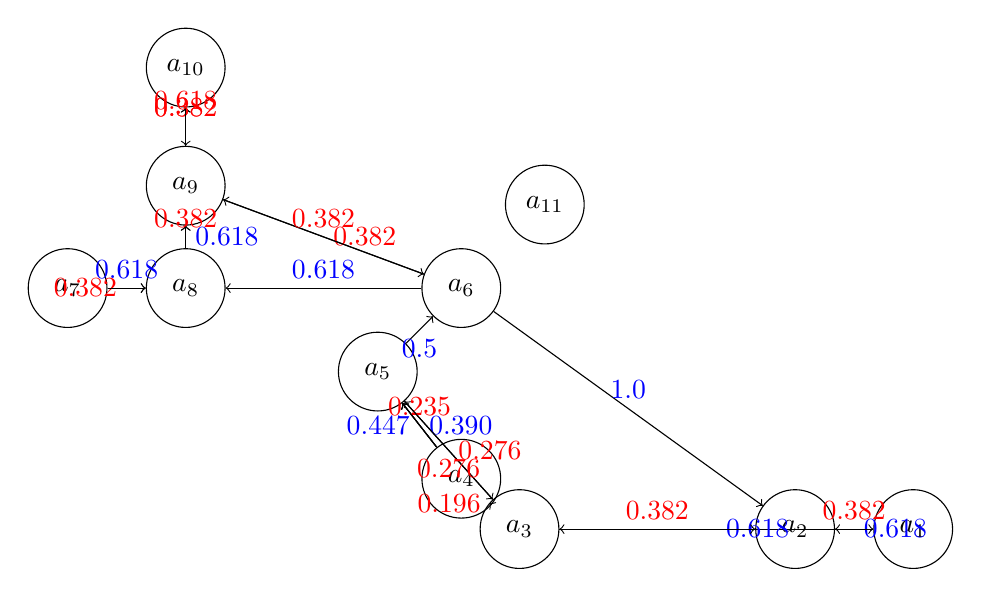
\begin{tikzpicture}[node distance=1.5cm, auto]
    \tikzset{vertex/.style = {shape=circle,draw,minimum size=1cm}}
    
    \node[vertex] (a7) {$a_7$};
    \node[vertex] (a8) [right of=a7] {$a_8$};
    \node[vertex] (a9) [above of=a8,yshift=-0.2cm] {$a_9$};
    \node[vertex] (a10) [above of=a9] {$a_{10}$};
    \node[vertex] (a6) [right of=a8,xshift=2cm] {$a_{6}$};
    \node[vertex] (a5) [below left of=a6] {$a_{5}$};
    \node[vertex] (a4) [below right of=a5,yshift=-0.3cm] {$a_{4}$};
    \node[vertex] (a11) [above right of=a6] {$a_{11}$};
    \node[vertex] (a3) [right of=a5,yshift=-2cm,xshift=0.3cm] {$a_{3}$};
    \node[vertex] (a2) [right of=a3,xshift=2cm] {$a_{2}$};
    \node[vertex] (a1) [right of=a2] {$a_{1}$};

    % Draw edges and annotations
    \path[->]
        (a7) edge node [left, red] {0.382} (a8)
        (a8) edge node [right, blue] {0.618} (a9)
        (a9) edge node [above, red] {0.382} (a10)
        (a9) edge node [right, red] {0.382} (a6)
        (a6) edge node [above, blue] {1.0} (a2)
        (a2) edge node [above, red] {0.382} (a1)
        (a1) edge node [right, blue] {0.618} (a2)
        (a1) edge node [right, blue] {0.618} (a3)
        (a3) edge node [above, red] {0.382} (a2)
        (a3) edge node [right, red] {0.276} (a5)
        (a4) edge node [right, blue] {0.390} (a5)
        (a4) edge node [above, red] {0.235} (a5)
        (a4) edge node [left, red] {0.196} (a3)
        (a4) edge node [left, blue] {0.447} (a5)
        (a5) edge node [below, blue] {0.5} (a6)
        (a5) edge node [below, red] {0.276} (a3)
        (a6) edge node [above, blue] {0.618} (a8)
        (a6) edge node [above, red] {0.382} (a9)
        (a7) edge node [above, blue] {0.618} (a8)
        (a8) edge node [above, red] {0.382} (a9)
        (a9) edge node [above, red] {0.382} (a10)
        (a10) edge node [above, red, pos=0.3] {0.618} (a9);
\end{tikzpicture}

\end{document}